% Options for packages loaded elsewhere
\PassOptionsToPackage{unicode}{hyperref}
\PassOptionsToPackage{hyphens}{url}
\documentclass[letterpaper,twocolumn,oneside,titlepage]{book}

\renewcommand{\familydefault}{ptm} % Set default font family to Times New Roman
\usepackage[nobottomtitles*]{titlesec}
\usepackage{tikz}
\usepackage{graphicx}
\usepackage[tc]{titlepic}
\usepackage{pgothic}
\usepackage[T1]{fontenc}
\usepackage{titlesec}

\titleformat{\chapter}[display]
    {\pgothfamily\huge\color{black}}
    {}
    {20pt}
    {}
\titlespacing*{\chapter}
    {0pt}
    {-10pt}
    {20pt}

%Set Background
\AddToHook{shipout/background}{%page backgrounds
    \put (0in,-\paperheight){
\includegraphics[width=\paperwidth,height=\paperheight]{img/style/background.jpg}}%
}

\title{
    
\includegraphics[width=\textwidth]{img/style/bg40klogo.png}\\
}


\usepackage{xcolor}
\usepackage{amsmath,amssymb}
\setcounter{secnumdepth}{5}
\usepackage{iftex}
\ifPDFTeX
  \usepackage[T1]{fontenc}
  \usepackage[utf8]{inputenc}
  \usepackage{textcomp} % provide euro and other symbols
\else % if luatex or xetex
  \usepackage{unicode-math} % this also loads fontspec
  \defaultfontfeatures{Scale=MatchLowercase}
  \defaultfontfeatures[\rmfamily]{Ligatures=TeX,Scale=1}
\fi
\usepackage{lmodern}
\ifPDFTeX\else
  % xetex/luatex font selection
\fi
% Use upquote if available, for straight quotes in verbatim environments
\IfFileExists{upquote.sty}{\usepackage{upquote}}{}
\IfFileExists{microtype.sty}{% use microtype if available
  \usepackage[]{microtype}
  \UseMicrotypeSet[protrusion]{basicmath} % disable protrusion for tt fonts
}{}
\makeatletter
\@ifundefined{KOMAClassName}{% if non-KOMA class
  \IfFileExists{parskip.sty}{%
    \usepackage{parskip}
  }{% else
    \setlength{\parindent}{0pt}
    \setlength{\parskip}{6pt plus 2pt minus 1pt}}
}{% if KOMA class
  \KOMAoptions{parskip=half}}
\makeatother
\usepackage{graphicx}
\makeatletter
\newsavebox\pandoc@box
\newcommand*\pandocbounded[1]{% scales image to fit in text height/width
  \sbox\pandoc@box{#1}%
  \Gscale@div\@tempa{\textheight}{\dimexpr\ht\pandoc@box+\dp\pandoc@box\relax}%
  \Gscale@div\@tempb{\linewidth}{\wd\pandoc@box}%
  \ifdim\@tempb\p@<\@tempa\p@\let\@tempa\@tempb\fi% select the smaller of both
  \ifdim\@tempa\p@<\p@\scalebox{\@tempa}{\usebox\pandoc@box}%
  \else\usebox{\pandoc@box}%
  \fi%
}
% Set default figure placement to htbp
\def\fps@figure{htbp}
\makeatother
\setlength{\emergencystretch}{3em} % prevent overfull lines
\providecommand{\tightlist}{%
  \setlength{\itemsep}{0pt}\setlength{\parskip}{0pt}}
\usepackage{bookmark}
\IfFileExists{xurl.sty}{\usepackage{xurl}}{} % add URL line breaks if available
\urlstyle{same}
\hypersetup{
  hidelinks,
  pdfcreator={LaTeX via pandoc}}

\author{Beta v1.0}
\date{\today}

\begin{document}
\frontmatter
\maketitle

{
\setcounter{tocdepth}{2}
\tableofcontents
\cleardoublepage
}
\mainmatter
\emph{Author's note:}\\
\emph{The following is designed to amend any edition of the Warhammer
40k rules.}

\emph{These rules are written with 7th in mind, but are intentionally
edition-agnostic where possible. Profiles and mechanics from any edition
may be used with minimal alteration in many cases.}

\emph{The usual movement, shooting, assault phases are replaced with an
interactive orders system instead. Voice of Command (Imperial Guard)
orders are their own still, these rules will not refer to them unless
explicitly stated otherwise}

\chapter{\texorpdfstring{\textbf{The Turn}}{The Turn}}\label{the-turn}

The standard Warhammer 40k turn structure is replaced with the
following:

\begin{enumerate}
\def\labelenumi{\arabic{enumi}.}
\tightlist
\item
  Start \& Reserves\\
\item
  Orders Phase\\
\item
  Assault Phase\\
\item
  Rally \& End
\end{enumerate}

\section{\texorpdfstring{\textbf{Start of
Turn}}{Start of Turn}}\label{start-of-turn}

Resolve any triggers or effects that would occur during the start of a
player or game turn. If an ability would trigger at the start of the
movement phase, it triggers at the start of the turn instead.

If using 7th edition, generate warp charges as if it were the start of
the psychic phase.

\section{\texorpdfstring{\textbf{Orders}}{Orders}}\label{orders}

During the turn, a player may issue each a single order in sequence,
until all units have acted or passed. An order must be fully resolved
before another is issued.

When issuing a reaction order, the unit should be marked with an
appropriate token to designate that it is waiting to carry it out. The
order may be declared and ``spent'' later on. Remove the token at the
start of the reaction order's resolution.

When resolving an order, treat each step as its own phase. Any ability
that would trigger during one of these phases triggers during the
relevant step of the order instead.

Reaction orders may be carried out at any point during the game, and a
reaction order may be performed as a response to another reaction order.
Resolve these in last-in, first-out order.

Unless noted otherwise, a step of an order as it would normally occur
during a gameplay phase (movement, shooting, etc.) must be fully
completed before the next one resolves. Abilities that would trigger at
the beginning or end of the movement or shooting phase trigger at that
time of the Orders phase instead.

\subsection{\texorpdfstring{\textbf{Top
Speed}}{Top Speed}}\label{top-speed}

The unit may move or disembark from a transport the normal distance,
plus the distance for running or moving flat-out.

\subsection{\texorpdfstring{\textbf{Maneuver and
Fire}}{Maneuver and Fire}}\label{maneuver-and-fire}

The unit moves or disembarks up to its movement allowance and makes a
shooting attack. This may be done in any order, but each action must be
fully completed before starting the next. Units that fire before moving
must fire as if

\subsection{\texorpdfstring{\textbf{Open
Fire}}{Open Fire}}\label{open-fire}

The unit fires once as it normally would during the shooting phase with
no penalties taken from movement. If the unit is not Gone to Ground, it
may shoot as though it had Split Fire.

\subsection{\texorpdfstring{\textbf{Close
Assault}}{Close Assault}}\label{close-assault}

The Maneuver and Fires, then may follow the standard procedure for
resolving a charge.

If a unit could fire overwatch, ignore these rules. Units on Ambush Fire
may carry out that order during the Charge Sub-phase instead.

\subsection{\texorpdfstring{\textbf{Request
Support}}{Request Support}}\label{request-support}

HQ units, or any character with Scout may attempt to request off-map
support. The unit targets an enemy, or a point on the map as if it were
a shooting attack.

The unit may select a single friendly off-map Barrage unit or selection
taken from Additional Fire Support and attempt a communications test
(Ld). The unit may perform no other action this turn as it relays
coordinates and directs fire.

If the communications test is passed, the support unit may perform an
order as described in the rules for Support Strikes. If the test is
failed, the order ends with no further resources spent.

Eligible units that are embarked on a transport may use this order if
they could normally fire from that transport and that transport remains
stationary for the turn.

\subsection{\texorpdfstring{\textbf{Tactical
Coordination}}{Tactical Coordination}}\label{tactical-coordination}

HQ Units only. The command unit can do nothing else this turn, but may
nominate a friendly unit anywhere on the table that has Gone to Ground
or routed to attempt to Rally or stand up. The unit must pass a
leadership test.

\subsection{\texorpdfstring{\textbf{Ambush Fire (Reaction
Order)}}{Ambush Fire (Reaction Order)}}\label{ambush-fire-reaction-order}

Mark the unit with any appropriate marker. The waiting ambush unit may
now interrupt any enemy unit's order to use their Open Fire order.

\subsection{\texorpdfstring{\textbf{Reserve Move (Reaction
Order)}}{Reserve Move (Reaction Order)}}\label{reserve-move-reaction-order}

A unit given the Reserve Move order does not move in its own turn but
instead waits, and can then interrupt the enemy turn (but not an order)
to take the Top Speed order

If a unit would reserve move after a shooting attack is declared but
before it is performed, the firing unit may choose to change targets
after the reserve move is resolved.

If the moved unit is out of range or line of sight, the firing unit may
fire snap shots at the target as if it were at any point along its
movement path.

Note: In general, orders or abilities that allow for an interrupt
resolve at any point during movement, or before/after a shooting attack
or other action is resolved.

\section{\texorpdfstring{\textbf{Assault
Phase}}{Assault Phase}}\label{assault-phase}

Resolve the Assault phase as the Warhammer 40k Fight Sub-phase. Units
may ignore restrictions for charging out of reserves.

\section{\texorpdfstring{\textbf{Rally \& End
turn}}{Rally \& End turn}}\label{rally-end-turn}

Routing units may attempt to rally as normal, except for units that
routed as the result of a combat resolution on the Assault Phase of this
turn.

Units belonging to the active player that have Gone to Ground may stand
up.

Resolve any other effects that would resolve at the end of a turn.

\chapter{\texorpdfstring{\textbf{Core
Rules}}{Core Rules}}\label{core-rules}

\section{\texorpdfstring{\textbf{Barrage}}{Barrage}}\label{barrage}

Units firing indirectly using Barrage use the following procedure
instead. Indirect Fire must be resolved using a Request Support order

Artillery units with a Barrage weapon may elect to be deployed off-map.
Units deployed this way may only fire indirectly, and may not draw Line
of Sight to any unit on the table. They do not count toward a player's
unit count.

A player may purchase a Pre-registered Target Point for 15 points as an
Additional Fire Support choice. An artillery battery may choose to fire
on this point without requiring a Request Support order. Spotter rounds
targeting this area deviate as normal. Pre-registered Target Points are
noted after Fortifications are deployed, but before any units are set
up.

\textbf{1. Position Spotter Round}\\
Place a spotter round marker anywhere on the table within the spotter's
line of sight and within 48'' of the spotter.

\textbf{2. Spotter Round Deviation}\\
The spotter round scatters 3D6''. If a direct hit is rolled on the
scatter die, remove the highest die. This distance may be reduced by the
spotter's Ballistics Skill.

\textbf{3. Fire for Effect}\\
Resolve each attack from the battery with Pinning as the corresponding
blast size, hitting the unit closest to the spotter round on 6+ instead
of 4+. For cover, draw Line of Sight from the spotter round's marker.
Blast modifiers apply.

\section{\texorpdfstring{\textbf{Deep
Strike}}{Deep Strike}}\label{deep-strike}

If a unit would be brought in using deep strike, instead place a deep
strike marker. This marker scatters following the rules for the unit
itself.

If the marker or unit would land in a location that would result in a
Mishap, roll on the table as normal. The Marker is not a unit, but
follows all rules for unit placement as if it were.

At the beginning of the player's following turn, replace the marker with
the first model in the unit as normal. The unit may receive orders as if
it had been on the board for a full turn. The unit counts as having
moved for the purposes of any abilities.

\subsection{\texorpdfstring{\textbf{Mishap}}{Mishap}}\label{mishap}

If the marker or any model in the unit would land in a location that
would result in a mishap, the opposing player may select one of the
following options:

\begin{itemize}
\tightlist
\item
  \textbf{Delayed:} The unit re-enters reserves until the start of the
  next game turn\\
\item
  \textbf{Misplaced:} The opposing player may choose a valid placement
  for the unit within 18'' of the center of the Deep Strike marker.
\end{itemize}

\section{\texorpdfstring{\textbf{Fearless}}{Fearless}}\label{fearless}

All Fearless non-vehicle units use the rules for And They Shall Know No
Fear instead. If another rule would normally affect a fearless unit,
that rule still applies to that unit.

Monstrous Creatures that lose 25\% of their wounds in a single turn must
take a Morale test as if it took 25\% casualties. If a Monstrous
Creature would fail a pinning test, it falls back instead.

\section{\texorpdfstring{\textbf{Flyers}}{Flyers}}\label{flyers}

Any unit with the Flyer type may only be used in hover mode and treated
as a Fast Skimmer, unless it (or any Fast Skimmer mutually agreed upon
to have the ability to act as a Flyer) is taken as a Support Strike.

Flyers that could otherwise zoom may only be charged by units with Jump
Packs, Jet Packs or other flyers.

\section{\texorpdfstring{\textbf{Go To
Ground}}{Go To Ground}}\label{go-to-ground}

Units may go Go to Ground at any point during an attack. They gain +2 to
their cover save and a 4+ unmodifiable cover save in the open, but fight
at WS 1 in melee while Gone to Ground.

Units that have Gone to Ground may perform an Open Fire order to fire
snap shots, but may perform no other actions.

\section{\texorpdfstring{\textbf{Morale
Re-rolls}}{Morale Re-rolls}}\label{morale-re-rolls}

If an ability would allow a unit to re-roll a failed Morale or Pinning
test, that ability may not be used again until the beginning of the next
turn.

\section{\texorpdfstring{\textbf{Point
Blank}}{Point Blank}}\label{point-blank}

Shooting attacks made within 6'' of their target and on the same level
of ruins (or top level for flyers) gain Ignores Cover, unless that unit
declared Go to Ground or Jink against this attack. (Units that are Gone
to Ground or Jinking as the result of another attack do not gain the
benefit of cover)

\section{\texorpdfstring{\textbf{Psychic
Manifestation}}{Psychic Manifestation}}\label{psychic-manifestation}

Psykers may attempt to cast a psychic power as if it were the psychic
phase at any point during an order. This may be done instead of moving
or shooting as part of another order. Spend warp charges or take tests
as usual, if relevant.

\section{\texorpdfstring{\textbf{Support
Strikes}}{Support Strikes}}\label{support-strikes}

A unit taken from Additional Fire Support may be called in to perform
one of the following via a Request Support order.

\subsection{\texorpdfstring{\textbf{Long-Range
Bombardment}}{Long-Range Bombardment}}\label{long-range-bombardment}

Artillery units may be taken as a battery or squadron for 10\% of their
normal cost. They may be called upon to use an Open Fire order that is
treated as One Use Only per battery. A unit that fires this way must
follow the procedure outlined in the Barrage section.

\subsection{\texorpdfstring{\textbf{Death From The
Skies}}{Death From The Skies}}\label{death-from-the-skies}

Single-model Flyer units may be taken for 20\% of their usual points
cost. This does not count toward a player's unit count for the purposes
of counting objectives.

Flyers with Transport Capacity may carry units embarked upon it declared
before the start of the game. Units that disembark from a zooming Flyer
ignore any replacement effects for Deep Strike markers and are deployed
immediately, treating any Mishap results as Misplaced.

Support Flyers enter the controlling player's board edge, and
immediately perform a Maneuver and Fire order. The Flyer may move up to
any point wholly within the controlling player's half of the board
treated as having moved Combat Speed, or anywhere on the opponent's half
as Cruising Speed. All other rules for Zooming Flyers apply.

During the end phase, remove the flyer from the board. Flyers that leave
the board this way are not counted as a casualty, but may not return to
the board. They are still counted as a casualty if they are destroyed by
other causes.

\section{\texorpdfstring{\textbf{Sweeping
Advance}}{Sweeping Advance}}\label{sweeping-advance}

After winning combat, units automatically attempt a Sweeping Advance if
eligible.

\subsection{\texorpdfstring{\textbf{Restrain or
Pursue}}{Restrain or Pursue}}\label{restrain-or-pursue}

The winning player may attempt to restrain the unit by passing a morale
test. If the attempt is failed or the unit does not attempt to restrain,
make the initiative test for Sweeping Advance as normal.

\subsection{\texorpdfstring{\textbf{CAUGHT!}}{CAUGHT!}}\label{caught}

If the chasing unit wins, the retreating unit suffers a number of wounds
equal to double the model count of the chasing unit with no saves of any
kind. Bulky and other rules that affect transport capacity may be
counted toward a unit's model count as it would for a transport.

\subsection{\texorpdfstring{\textbf{Move Fleeing
Unit}}{Move Fleeing Unit}}\label{move-fleeing-unit}

If the fleeing unit was not destroyed, it falls back.

\subsection{\texorpdfstring{\textbf{Follow-up
move}}{Follow-up move}}\label{follow-up-move}

Move the pursuing unit its own Fall Back distance toward the fleeing
unit. If the pursuing unit successfully caught its target, they may move
within 1'' of the fleeing unit and combat continues. Otherwise, move
them up to, but not within 1''.

\section{\texorpdfstring{\textbf{Tank
Riders}}{Tank Riders}}\label{tank-riders}

Riding a tank beats walking. A Tank that does not already have a
transport capacity may carry up to 4 Infantry models per hull point as
Tank Riders (as if it were a transport.)

Infantry units with a 4+ save or lighter may be deployed as Tank Riders.
A tank and its riders count as a single unit for purposes of deployment
and reserves, as if it were a transport. They are treated exactly as
transport passengers, but are far more exposed.

Tank Riders may be targeted separately from the vehicle, may be Pinned
separately, and count as having 5+ cover. If the unit would Go to
ground, they immediately disembark.

If the transporting tank is hit by fire that could remove a hull point,
the riding unit is immediately disembarked and treated as if they had
failed a pinning test. If the vehicle is destroyed while they are
embarked, d3 models are removed with no saves of any kind allowed.

\section{\texorpdfstring{\textbf{Templates}}{Templates}}\label{templates}

Templates use the following rolls to hit, noted as (number of dice) /
(to-hit):

\begin{verbatim}
Small Blast 3 / 4+  
Large Blast 6 / 4+  
Flame       6 / 4+ (6” Range)
\end{verbatim}

Template weapons of any kind may not inflict more hits than there are
models in a unit. Discard excess hits.

If a target unit has double the number of models or more compared to a
weapon's dice pool to hit, template weapons gain an additional +1 to
hit.

If the target unit did not move after the start of the previous turn,
template weapons gain an additional +1 to hit.

If a target unit is in cover, flame weapons get an additional +1 to hit

If another unit is within 3'' of a target being hit by a blast weapon,
or 6'' for a large blast, to-hit rolls of 1 hit that unit instead. If
multiple units are in the same whole number of inches apart
(e.g.~between 3 and 4''), randomly allocate these hits to each unit.

\section{\texorpdfstring{\textbf{Transports}}{Transports}}\label{transports}

Infantry may declare a disordered charge out of a transport that does
not have the Assault Vehicle special rule if that transport did not move
this turn. A transport that had infantry disembark this way may not move
for the rest of the turn.

\section{\texorpdfstring{\textbf{Vehicle
Squadrons}}{Vehicle Squadrons}}\label{vehicle-squadrons}

Vehicles may be taken as a squadron as part of Force Organization, and
are treated as completely separate units otherwise.

\section{\texorpdfstring{\textbf{Wound
Allocation}}{Wound Allocation}}\label{wound-allocation}

The player targeted by an attack or ability that could cause wounds may
choose which model to allocate wounds of any type, unless specified by
another rule. For units with mixed saves, this must be declared before
rolling saves of any kind. Wounds must be allocated to models already
wounded.

Look out Sir! may not be used against wounds of any kind.

\chapter{\texorpdfstring{\textbf{Force
Organization}}{Force Organization}}\label{force-organization}

Instead of the usual Combined Arms and other Formation detachments, army
lists must conform to the Battlegroup detachment configuration as
described below. An army composed this way gains the same benefits as if
it were a Combined Arms detachment.

\section{\texorpdfstring{\textbf{Allies}}{Allies}}\label{allies}

Any army may include selections from another army selection rated as
Battle Brothers as part of the same Battlegroup detachment.

Slots enabled from a given selection must be taken from the same faction
list. (e.g.~an Imperial Guard troop may only unlock slots for Imperial
Guard units)

Allies that are not Battle Brothers may be taken as a single separate
Battlegroup detachment.

\section{\texorpdfstring{\textbf{Frontline
Assets}}{Frontline Assets}}\label{frontline-assets}

HQ and Troops units may be taken in any quantity, following any other
limitations for list building.

\subsection{\texorpdfstring{\textbf{HQ}}{HQ}}\label{hq}

For each HQ unit taken in your roster, you may include a single unit
from Elites or Additional Fire Support.

HQ units may not exceed 25\% of an army's total point limit.

\subsection{\texorpdfstring{\textbf{Troops}}{Troops}}\label{troops}

For each Troops unit taken, you may include a single unit from Elites,
Fast Attack, or Heavy Support.

One Troop unit must be taken per 1000 points.

\section{\texorpdfstring{\textbf{Support
Assets}}{Support Assets}}\label{support-assets}

These are specialist units, and may only be taken in limited quantities.
Elites, Heavy Support, and Fast Attack units may only be taken as
described below:

\subsection{\texorpdfstring{\textbf{Fast
Attack}}{Fast Attack}}\label{fast-attack}

Each unit taken from Fast Attack allows a support choice from Additional
Fire Support.

\subsection{\texorpdfstring{\textbf{Heavy
Support}}{Heavy Support}}\label{heavy-support}

Heavy Support units composed entirely of Infantry models may be taken as
a Troops unit.

Units taken this way do not receive any bonuses or provide an additional
force organization slot as regular troops would, and do not fulfill the
compulsory requirements for troops.

Troops slots filled this way may not outnumber slots filled by standard
Troops.

\subsection{\texorpdfstring{\textbf{Fortifications}}{Fortifications}}\label{fortifications}

Fortifications may only be taken by the defender in an Attack/Defense
scenario, in any quantity. It is recommended to determine the scenario
before lists are written to account for this.

\subsection{\texorpdfstring{\textbf{Additional Fire
Support}}{Additional Fire Support}}\label{additional-fire-support}

Any Artillery or Flyer unit may be used in a support role for a fraction
of its normal points value. These units are not deployed on the map
normally, nor placed in reserves. Refer to the Support Strike section
for full details.

\subsection{\texorpdfstring{\textbf{Lords of
War}}{Lords of War}}\label{lords-of-war}

One Lord of War may be taken in place of a Heavy Support for every full
3000 points in the game's limit.

\subsection{\texorpdfstring{\textbf{Restricted
Units}}{Restricted Units}}\label{restricted-units}

Restricted units and wargear are rare items to which an army just would
not have easy access. Restricted units are limited by the size of a
game. Players may take only one restricted unit or wargear option per
1000 points,unless a scenario or special rule would apply otherwise.

The following units (and wargear) are considered to be Restricted:

\begin{itemize}
\tightlist
\item
  Relics (or Relics of the Armoury)\\
\item
  Vehicles with 5 or more Hull Points\\
\item
  Monstrous Creatures with 5 or more Wounds\\
\item
  Grav \& Graviton Weapons\\
\item
  Lords of War
\end{itemize}

\chapter{\texorpdfstring{\textbf{Scenario
Rules}}{Scenario Rules}}\label{scenario-rules}

\section{\texorpdfstring{\textbf{Objectives}}{Objectives}}\label{objectives}

Objectives have a 3'' capture radius, and control may be denied by any
eligible units within 6''. (Objective Secured, for example)

Standard objectives must be placed at least 12'' apart and 12'' away
from any table edges unless otherwise noted.

The point must be in line of sight of a unit to capture or deny, in
addition to any other restrictions.

\subsection{\texorpdfstring{\textbf{Out-Scouted}}{Out-Scouted}}\label{out-scouted}

If one player deployed more Recon units, that player may claim the
Out-Scouted secondary objective for 1VP

\section{\texorpdfstring{\textbf{Reconnaissance
Units}}{Reconnaissance Units}}\label{reconnaissance-units}

Scenarios may refer to Reconnaissance (or Recon) units. Unless otherwise
specified, the following unit types are considered Recon units:

\begin{itemize}
\tightlist
\item
  Non-Flyer Fast Attack\\
\item
  Units with Scout or Infiltrate
\end{itemize}

\section{\texorpdfstring{\textbf{Victory
Conditions}}{Victory Conditions}}\label{victory-conditions}

In addition to any scenario rules, if a player controls all objectives,
or the opponent controls no units that are not Gone to Ground or
routing, they win the game. Fortifications alone do not count for units
remaining on the table.

\section{\texorpdfstring{\textbf{VP
Limits}}{VP Limits}}\label{vp-limits}

Some scenarios will use a VP limit instead of the usual scoring. A
recommended VP limit for a given scenario is triple the number of
objectives on the field, plus the average unit count of both or all
players.

When an objective is captured, VPs are awarded immediately. If a point
that was previously captured is seized by an enemy, these VPs are not
lost.

\section{\texorpdfstring{\textbf{Turn 0}}{Turn 0}}\label{turn-0}

Some scenarios include a Turn 0, where reconnaissance units may operate
before events that would normally occur during the first turn of the
game.

\chapter{Scenarios}\label{scenarios}

\section{Counter-Attack}\label{counter-attack}

\begin{figure}
\centering
\pandocbounded{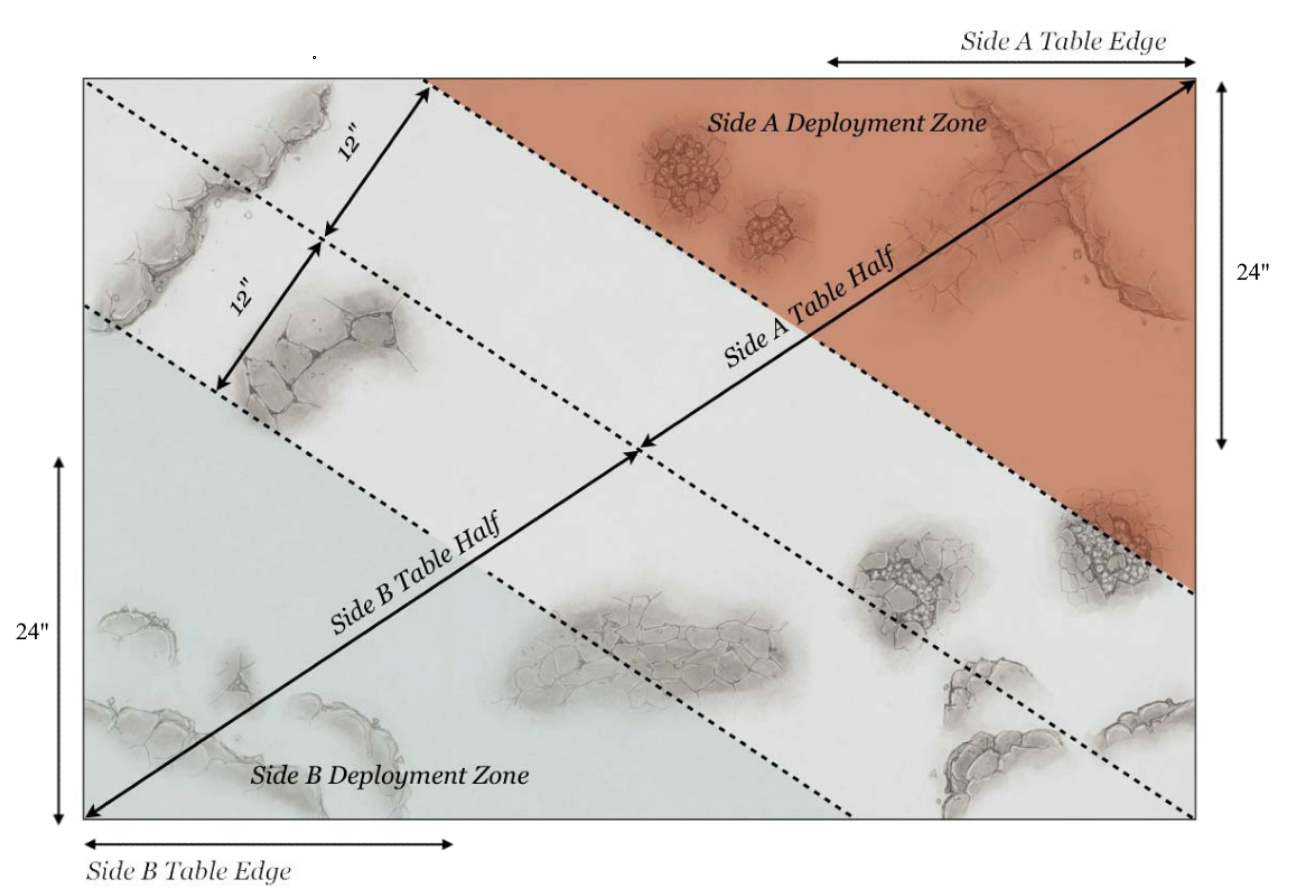
\includegraphics[keepaspectratio]{img/Counter-Attack.png}}
\caption{Deployment Map}
\end{figure}

\textbf{SITUATION REPORT}\\
An enemy attack has broken through which may force a withdrawal of
troops at the front. Your battlegroup has been held in reserve to
counter. Move fast to intercept and halt the enemy breakthrough. Both
sides are on the move, there is little time for preparation.

\textbf{Scenario Type}: Meeting Engagement

\textbf{TERRAIN}\\
Set up the terrain in any mutually agreed manner.

\textbf{VICTORY}\\
Victory Points are scored cumulatively until the VP limit is reached:\\
Capturing an Objective (+3VP)\\
Enemy Unit slain (+1VP)\\
Slay the Warlord (+1VP)\\
Out-Scouted (+1VP)

The recommended VP limit is triple the number of objectives on the
field, plus the average unit count of all players rounded down.

\textbf{DEPLOYMENT}\\
\textbf{1. Determine table corners}\\
Both sides roll a D6 and add the number of Recon units in their army.
The player with the highest total chooses which table corner will be his
deployment zone, the opponent automatically gets the opposite table
corner.

\textbf{2. Place Objectives}\\
Place D3+2 objectives on the table. The side that chose deployment zones
places the first, then both sides alternate placement.

\textbf{3. Reconnaissance Forces}\\
Players alternate deploying all Recon units in the same order. These can
be placed anywhere in their half of the table, but not within 12'' of
the table's centerline. Units alternate Infiltrate deployments after all
other units are placed.

Recon units may be declared held in reserves instead of deploying. The
side that deployed more Recon units may claim the Out-Scouted secondary
objective.\\
If one side has deployed no units, then the opponent may position their
units anywhere on the table on Ambush Fire.\\
\textbf{4. Turn 0}\\
Both players roll a D6 adding the number of units deployed in step 3.
The side with the highest total takes the first turn. On a tie, the side
that deployed the most Recon units wins.

\textbf{5. Main Force Arrival}\\
From turn 1 onwards, players bring in units from reserves equal to the
turn number. Units entering the board may be placed fully within 6'' of
the player's table edge (24'' each direction from the table corner).
Continue this until all the forces are on the tabletop.

*For every 2000 points of game size, roll an additional D3 \pagebreak

\section{Defense Line}\label{defense-line}

\pandocbounded{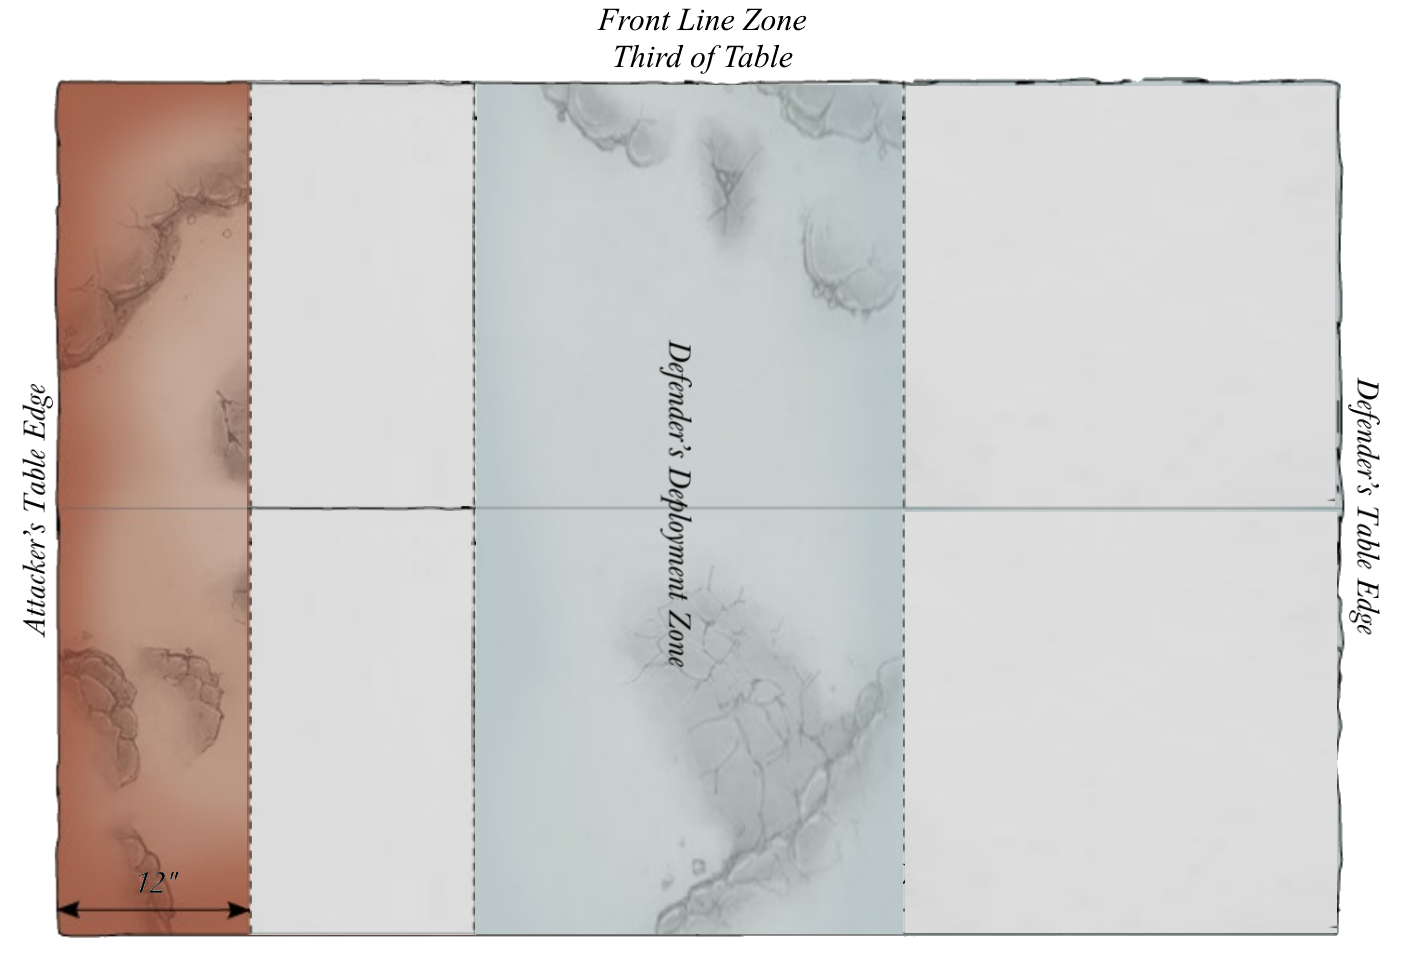
\includegraphics[keepaspectratio]{img/DefenseLine.png}}
\textbf{SITUATION REPORT}\\
The enemy have already been under heavy artillery fire, and are already
weakened. Spearhead an assault to break through the lines.

\textbf{Scenario Type}: Attack/Defense

\textbf{TERRAIN}\\
Set up the terrain in any mutually agreed manner.

\textbf{VICTORY}\\
Victory Points are scored cumulatively until the VP limit is reached:\\
Capturing an Objective (+3VP)\\
Enemy Unit slain (+1VP)\\
Slay the Warlord (+1VP)\\
Out-Scouted (+1VP)

The recommended VP limit is triple the number of objectives on the
field, plus the average unit count of all players rounded down.

\textbf{RESERVES}\\
Reserves enter the table in waves. During the game, one unit, plus one
for every 1000 points of game limit will arrive as a wave where noted.

\textbf{1. Determine Table Edges}\\
The defender may choose which of the short table edges the Attacker must
deploy on. He gets the opposite table edge.

\textbf{2. Attacker's Forces}\\
\textbf{Probing Force}\\
The probing force must include all the Attacker's Recon units and one
wave of reserves as described above.

\textbf{Main Force}\\
The rest of the attacker's battlegroup are his main force. From turn 3
onwards, one wave will enter the board from the attacker's table edge at
the beginning of each turn.

\textbf{3. Determine Initial Defenders}\\
The defender may select up to half of their units, plus any
Fortifications to start. All other units are placed in reserves.

\textbf{4. Defender's Reinforcements}\\
From turn 5 onwards one wave will arrive each turn from his table edge,
until all units are on the tabletop.

\textbf{5. Objective Placement}\\
The defender places two objectives in the front line zone, and one
anywhere else on the table, with the usual restrictions. The defender
may not claim all objectives secured victory.

\textbf{6. Deploy Initial Defenders} Place all the initial defenders in
the front line zone. D3 units may start the game on the Ambush Fire
order.

\textbf{7. Deploy Attacker's Probing Force}\\
The attacker's probing force units are placed within 12'' of the
attacker's table edge.

\textbf{8. Resolve Bombardment}\\
Each of the defender's non-vehicle units must take a Pinning test.
Vehicles must pass a leadership check, or count as Crew Stunned at the
start of the game.

\textbf{10. First Turn}\\
The attacker takes the first turn. \pagebreak

\chapter{\texorpdfstring{\textbf{Codex
Changes}}{Codex Changes}}\label{codex-changes}

\section{\texorpdfstring{\textbf{Imperial
Guard}}{Imperial Guard}}\label{imperial-guard}

\textbf{Vox-Casters}: Units with a Vox-caster may Request Support if
they are in vox network with an eligible unit that could Request Support
and they did not receive a Voice of Command order this turn.

\textbf{Forward Sentries:} Veterans with this doctrine may be treated as
a Recon unit if they did not purchase a Dedicated Transport.

\section{\texorpdfstring{\textbf{Tyranids}}{Tyranids}}\label{tyranids}

\subsection{\texorpdfstring{\textbf{Special
Rules}}{Special Rules}}\label{special-rules}

\textbf{Synapse}: Creatures in Synapse range may use the highest
leadership of Synapse creatures in range

\textbf{Psychic Consonance}: Synapse creatures in Synapse range of other
Synapse creatures may be counted as having +1 Toughness for the purposes
of Instant Death.

\textbf{Synaptic Lapse}: If a Synapse creature fails a Morale or Pinning
test, its Synapse Range is reduced to 0'' until it Regroups or is no
longer Gone to Ground.

\chapter{\texorpdfstring{\textbf{Experimental
Rules}}{Experimental Rules}}\label{experimental-rules}

\section{\texorpdfstring{\textbf{Assault
Phase}}{Assault Phase}}\label{assault-phase-1}

\subsection{\texorpdfstring{\textbf{``Overwatch''}}{``Overwatch''}}\label{overwatch}

During the Charge Sub-Phase after Charge distance has been rolled, the
defending unit may elect to spend attacks from its Attacks
characteristic to fire weapons with a total range of 18'' or less. Units
that have Gone to Ground may not fire.

A model may make a shooting attack with a single Assault(X) weapon it
holds, or up to 2 Pistol weapons. If the charge was successful, treat
the range as 1''. The model's Attacks (A) characteristic is reduced by 1
for each shot until the end of the turn.

If the chosen weapon has a greater Assault(X) than the attacks
characteristic of the firing model, the model may still fire at a -1
penalty for each shot over the limit, to a minimum of 6+. This penalty
applies to all shots fired by the model.

Assault Weapons that are double the bearer's strength or higher may only
be fired as Snap Shots this way.

\emph{Example: A Fire Warrior with a pulse carbine fires 2 shots at -1
each, due to its A1 characteristic. Its Attack characteristic is reduced
to 0 for the rest of the turn, and may not attack during the Fight
sub-phase.}

\backmatter
\end{document}